\section{Teori}

Denne labben bestod av to forsøk, første del gikk ut på å gjøre målinger av en RC-krets ved hjelp av oscilloskop.
Med hensikt å analysere en kondensators effekt på et AC signal.
Andre del gikk ut på å analysere en CMOS krets med forskjellige inngangssignaler;
CMOS er en innfallsvinkel for å utvikle digitale kombinatoriske kretser.

\subsection{Teori del 1.}

    \begin{itemize}
        \item[-] Kondensator: En kondensator er en passiv elektrisk komponent viss bruksområde er å lagre elektrisk ladning.
        Den består av to elektroder skilt med et dielektrisk materiale.
        Et dielektrisk materiale har elektrisk isolerende egenskaper og polariseres når det påvirkes av et elektrisk felt.
        Kondensatorer beskrives symbolsk ved uttrykket $F = \frac{Q}{U}$, der $Q$ er ladning målt i Coulomb, $U$ er spenning målt i Volt og $F$ er kapasitansen målt i Fahrrad.
        Fahrrad tilsvarer altså Coulomb/Volt.
        Kapasitansen beskriver mengden elektroner som må tilføres elektrodene for å danne en gitt spenning over dem.
        \item[-] RC-Krets: En enkel RC-krets består av en motstand og en kondensator koblet i serie se figur (3-1 ish).
        Spenning over kondensatoren i en slik krets kan beskrives ved $v_{C}(t) = V_{kilde} \cdot \left( 1 - e^{-\frac{t}{\tau}} \right)$ under oppladning og $v_{C}(t) = V_{kilde} \cdot e^{-\frac{t}{\tau}}$ under utladning.
        Begge er uttrykt ved tiden $t$ gitt i sekunder, og gjelder for $t > 0$.
        $\tau = R \cdot C$, $R$ er motstand målt i Ohm, og $C$ er kapasitans målt i Fahrrad.
    \end{itemize}

\subsection{Teori del 2.}

    \begin{itemize}
        \item[-] PMOS-, og NMOS-transistor: De mest grunnleggende byggeklossene i logiske kretser er disse to formene for transistor, som begge fungerer som brytere.
        PMOS slipper signaler gjennom ved input: lav, og blokkerer dem ved input: høy.
        NMOS fungerer på samme måte, men invertert.
        Se~\ref{fig:pnmos_transistors} Ved bruk av disse kan man konstruere alle logiske porter.
    \end{itemize}

    \begin{figure}[!htb]
        \centering
        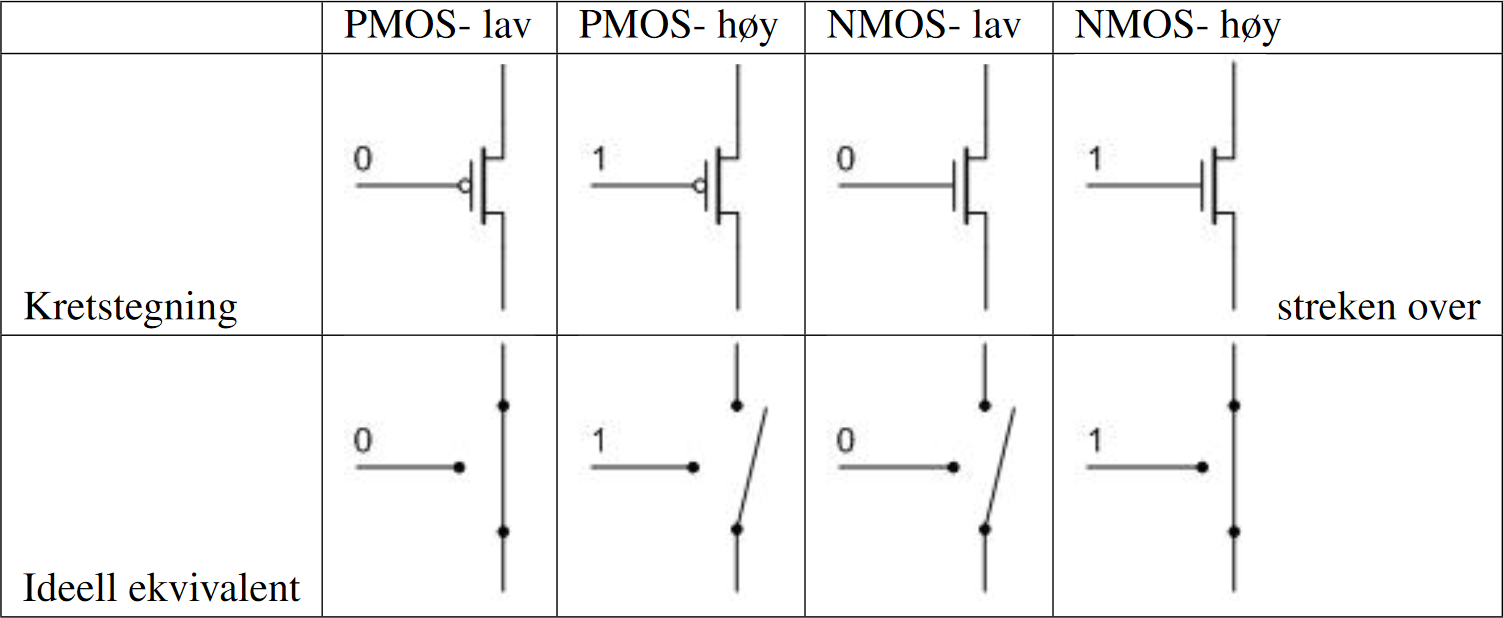
\includegraphics[height=6cm]{figurer/PNMOS.png}
        \caption{PMOS og NMOS- transistor med deres ideelle ekvivalenter for åpen og lukketkanal.}
        \label{fig:pnmos_transistors}
    \end{figure}

\begin{enumerate}
    \item Nummert
    \item Liste
    \begin{enumerate}
        \item Med Nøstede
        \item Elementer
    \end{enumerate}
\end{enumerate}

\begin{enumerate}[label=(\roman*)]
    \item Nummert
    \item Liste
    \begin{enumerate}[label=(\alph*)]
        \item Med Nøstede
        \item Elementer
        \begin{enumerate}[label=(\arabic*)]
            \item Og
            \item egne
            \item labels
        \end{enumerate}
    \end{enumerate}
\end{enumerate}



